\section{Interactive 3D graphics with Three.js}
\setauthor{Romeo Bhuiyan}
\textbf{Three.js}\cite{threejs} is a JavaScript library that allows for the creation of interactive 3D graphics in the web 
browser. It is designed to work seamlessly with WebGL, which is a web-based 3D graphics API that allows 
developers to access the hardware-accelerated graphics capabilities of a user's computer. Three.js 
makes it possible to create rich 3D experiences with JavaScript and HTML, without the need for any plugins or downloads.
With Three.js, developers can create a wide variety of 3D scenes and animations, including but not limited to: 
realistic environments with dynamic lighting and shadows, complex 3D models and animations, interactive 3D 
games and simulations, and virtual reality (VR) and augmented reality (AR) experiences.

The library provides a large number of powerful features and abstractions that simplify 
the process of creating 3D graphics. It includes a number of built-in shapes, such as cubes, 
spheres, and cylinders, as well as more complex shapes that can be constructed from the 
vertices and faces of custom 3D models. Three.js also includes a number of materials that 
allow for realistic shading and texturing of 3D objects, as well as lights and cameras 
that can be positioned and manipulated to achieve the desired lighting and perspective effects.
Another important aspect of Three.js is its support for keyframe animations. This allows
developers to animate objects over time, creating smooth transitions and movements. 
The library also provides support for physics simulations, making it possible to 
create complex and interactive 3D experiences that respond to user input.

\subsection{Rendering and manipulating VRM}
\setauthor{Romeo Bhuiyan}
\textbf{Three-vrm.js} is a JavaScript library that provides support for rendering 
and manipulating VRM (Virtual Reality Model) characters in web-based environments. 
It is built on top of Three.js, a widely-used library for creating 3D graphics and 
animations in web browsers.
Three-vrm.js offers a set of tools and APIs for working with VRM models, allowing 
developers to easily import, manipulate and animate VRM characters in their web-based 
projects. This includes support for importing VRM files, as well as manipulating and animating 
individual bones, rigging, morph targets, and materials of the characters as shown below in the figure \ref{fig:threevrmdebug}.
In addition to basic VRM functionality, three-vrm.js also includes a set of VRM-specific 
features and extensions. For example, it provides support for VRM's humanoids, which define 
the structure of a VRM character and allow for easy animation of the character. It also includes 
support for VRM's blend shapes, which are used to manipulate the shape of the character's 
face and expressions.
\\
\begin{figure}[htb]
    \centering
    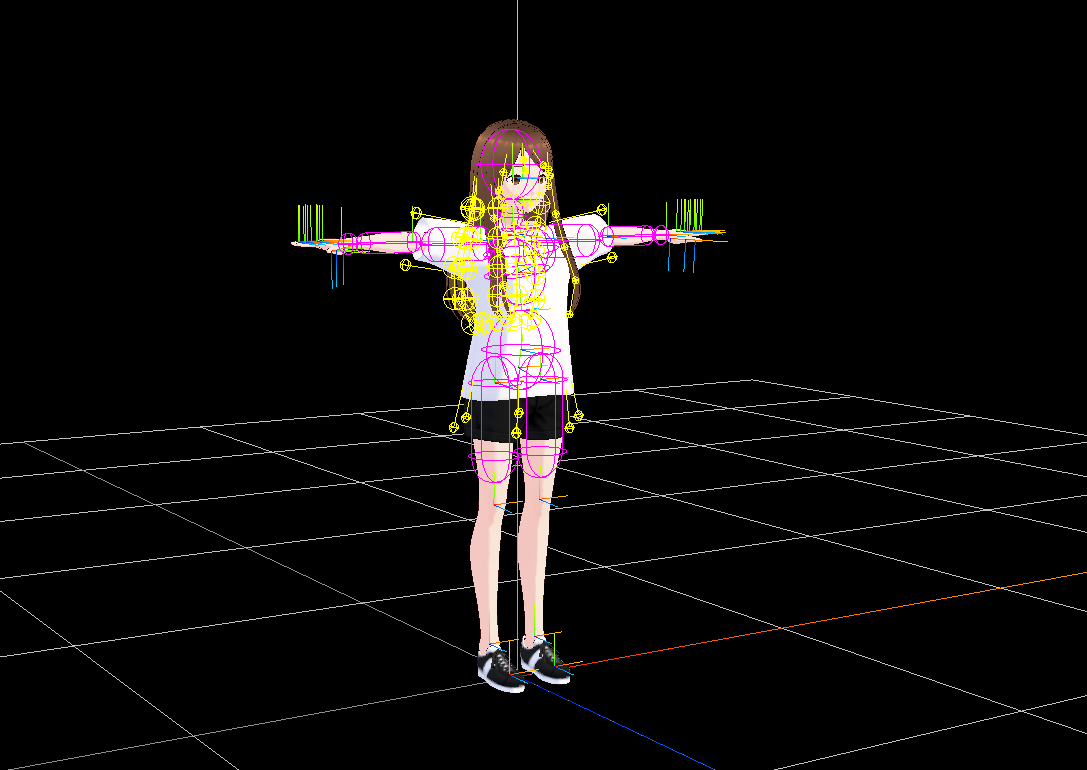
\includegraphics[width=0.9\textwidth]{pics/threevrmdebug.PNG}
    \caption{Three-vrm.js debug mode}
    \label{fig:threevrmdebug}
\end{figure}
\\
\section{Decision between web frameworks}
\setauthor{Christoph Lasinger}
The decision to use a web framework at all and not simply vanilla HTML, CSS and JavaScript came from a multitude of reasons.
For example, all the ways they provide assistance while developing, such as providing a file structure in which to neatly 
organize a project, a prebuilt routing system, a template-project that can serve as starting point, an option to debug a 
project and many more. As a result, a great amount of both time and effort can be saved, that can then in turn be spent on 
those particular parts of the project that are actually important.

Another reason to use web frameworks that has less to do with development, but more with working as a software engineer in 
the real world, is that for a lot of jobs experience in working with certain frameworks is certainly very useful, if not 
even required. The following graph \ref{fig:WebframeworkJobs} shows a breakdown of about 650 000 job offerings on websites like Linkedin, 
Dice and Glassdoor by the required framework \cite{WebframeworkJobs}.
\\
\begin{figure}[htb]
  \centering
  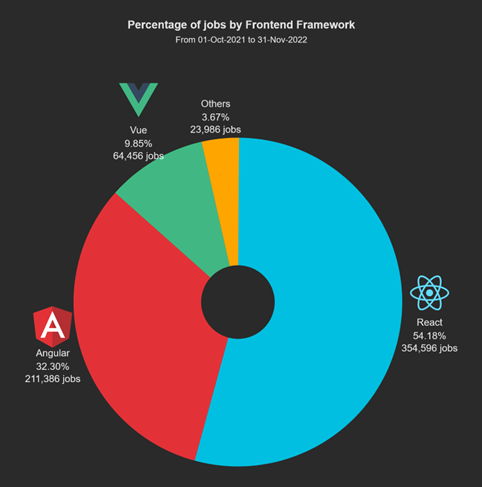
\includegraphics[width=0.7\textwidth]{pics/piechartwebframework.png}
  \caption{Breakdown of job offerings by framework}
  \label{fig:WebframeworkJobs}
\end{figure}
\\
\section{Angular}
\setauthor{Christoph Lasinger}
Angular, the next version of the discontinued AngularJS, is a framework for single-page applications (SPAs) and is maintained and released
by Google in 2016. An SPA is a type of web application that dynamically rewrites the current webpage instead of entirely reloading, i.e.,
requesting and displaying data from the server, it. The main benefits of SPAs are a more responsive user experience and avoiding the delay
of having to wait for a website to load. \cite{RoadToReact}
% is this really a good description of Angular?
\\
Angular is a free and open-source project, meaning that the copyright owner, in this case the company Google,
gives anyone the right to distribute, modify and study the software for any purpose. Open-source software is 
however not the same as public-domain software as it still possesses a copyright, just a very open one, hence its name. 
One big advantage of such software over closed-source software is that anyone in the world can find bugs and make 
improvements for it, free of charge for the actual project-owner. Moreover, even if the publisher decides to no longer 
provide support and update their software, it can still be adapted and improved by its users. Amazingly, it can be seen 
in practise that this concept works and users really do improve open-source projects not only for their benefit but for 
that of others as well. For those reasons, Animotion too is an open-source project \cite{Opensource}.
\\
Concretely, Angular is a web framework, built on Typescript, a high-level, object-oriented programming language that is 
a superset of JavaScript, that can be used to build from small projects to enterprise-grade web applications. It has a 
large library-collection that covers a wide array of features and offers an equally large number of developer tools for 
testing, updating and maintaining one's code. Moreover, Angular is component-based, meaning that an application consists 
of several building blocks (components), whereas each one defines one part of the user interface and any behaviour associated 
with it. Because these components are reusable and effectively modularize the application, it becomes easier to develop and 
test and makes the code more readable. This effect is especially noticeable in large-scale projects \cite{AngularDescription}.
\\
The Angular \gls{cli} plays a big part in development as it is used to efficiently and 
conveniently create, build, and test Angular applications by using the commands \texttt{ng new}, \texttt{ng build}
and \texttt{ng test} respectively. It can also be used to add new libraries through \texttt{ng add}
when needed. However, the most important command when developing is ng serve, as it starts the application on
localhost and automatically rebuilds it and reloads the website if any changes to the source code occur, which makes 
developing more convenient \cite{AngularCLI}.
\\
\section{React}
\setauthor{Christoph Lasinger}
Like Angular, React also is an open-source SPA-Framework, released by Meta (then Facebook) in 2013 and maintained by
Meta and a community of developers. Although the main focus of React lies on the component system and its DOM, it also 
has a large ecosystem of libraries surrounding it, making React flexible in terms of its uses.
% one more sentence?

\subsection{Virtual DOM}
\setauthor{Christoph Lasinger}
As mentioned before, among the most notable features of React is its virtual DOM (Document Object Model), a type of 
data structure that represents a webpage making it possible to only update certain parts of it that have changed. 
This provides a major performance boost but does not create extra effort for the developer as they can still write 
code as if the entire page is re-rendered on each refresh.

\subsection{Components}
\setauthor{Christoph Lasinger}
As React is a component-based framework, the feature of components is one of its main concepts. Concretely, they
allow the UI of a website to be split up into many reusable, independent parts,
for example a button, an input form, a dialog, and so on. In the programming language of React, JavaScript,
components can be either implemented through functions, so-called function components, or classes, which is done 
more commonly as they provide more features. In general, React components work like a function, they are handed 
arbitrary inputs which are called props in the terminology used by React
and return UI elements that are displayed on the website. When creating 
such a class the minimum requirements are that it extends the base component class React.Component, though it 
also possible to define one's own base class it is strongly discouraged in the official documentation of React,
and that it defines a method called render \cite{ReactComponentProps} \cite{ReactComponent}.
\\
\subsection{React JSX}
\setauthor{Christoph Lasinger}
React JSX is an abbreviation of JavaScript XML and a combination
of HTML and JavaScript. It plays a big part in React as JSX is the return type of all components. The following 
code snippet shown in listing \ref{lst:react} serves of an example.

\begin{lstlisting}[language=Python,caption=Example of a react component,label=lst:react]
  export default function About() {
  return (
    <>
    <button className="back-button" onClick={() => { GoTo("/"); }}>
      <p>back to menu</p>
    </button>
    <h1 id="main-headline" className="glitch" data-text="Community">Community</h1>
    <p className="community-text">
        Welcome to the community of Animotion! <br />
        Here you can join our official discord server and get to know new people. <br />
        You can also upload your own music and dance videos. <br />
        If you need help our 24/7 support is always here for you.
    </p>
    <iframe className="discord-iframe" src="https://discord.com/widget?id=1035647726634934382&theme=dark" allowtransparency="true" frameBorder="0" sandbox="allow-popups allow-popups-to-escape-sandbox allow-same-origin allow-scripts"></iframe>
    </>
  )
}
\end{lstlisting}

This exported function called About is, besides any imports that occur above it, practically the only code that makes 
up a so-called page, which exactly translate to a webpage, i.e., what comes up after visiting an URL. This function 
that shares its name with the file, a JavaScript file to be exact, merely consists of one long return statement that 
contains multiple HTML elements making up the webpage \cite{ReactJSX}.
The empty opening and closing tags at the beginning and end of the statement is the short syntax for a fragment, a 
feature in React that acts as a container and allows returning multiple child elements in a return statement 
without adding additional nodes to the DOM \cite{ReactFragments}.
\\
\subsection{Creating an Angular project}
\setauthor{Christoph Lasinger}
The easiest way to set up a React project is to use the officially supported command \emph{create-react-app}
(a similar command exists for Next.js, namely \emph{create next-app}) as it offers a modern build setup and is already preconfigured. 
Optionally, further parameters can be used to customize the project, for example \emph{—template typescript} to use TypeScript 
instead of JavaScript. After the project is created, it can immediately be started and viewed on localhost using either 
\emph{npm start} or \emph{yarn start}, depending on the package manager that is used. For development the command \emph{npm run dev} is 
also very useful, as the website is immediately refreshed after saving any changes to the code \cite{create-react}.
\\
\subsection{Comparison between Angular and React}
\setauthor{Christoph Lasinger}
In many regards React is similar to Angular, as they are both popular, component-based, open-source web frameworks. However, one 
significant difference that is especially important for beginners who have never worked with either one before lies in the 
steepness of their learning curves i.e., the one of Angular is much steeper than the one of React, meaning React is much easier 
to learn than Angular.

Additionally, in terms of popularity the gap between the two overall only seems to increase, with React coming out on top. This 
matters not only in the impact of demand on the job market but also in the size of the community. Because both projects are 
open-source a larger community means more active development, faster bug fixes, increased longevity, more chances of assistance 
in forums, and so on.

Another difference to consider when choosing one over the other is their respective programming language. While Angular is built
on TypeScript, React is a JavaScript library, so previous experience with one or the other, in case of TypeScript probably
more so the lack of experience, might influence the decision \cite{AngularReactComparison}.

While Animotion started out as an Angular project, after a short period of time we decided to use React instead, because it 
is easier to learn and more popular as well, as can be seen in figure \ref{fig:webpop} below. This graph shows the amount of 
searches for the npm packages of Angular represented in blue and React represented in orange in the past two years on
the npm trends website \cite{AngularReactPopularity}.
\\
\begin{figure}[htb]
  \centering
  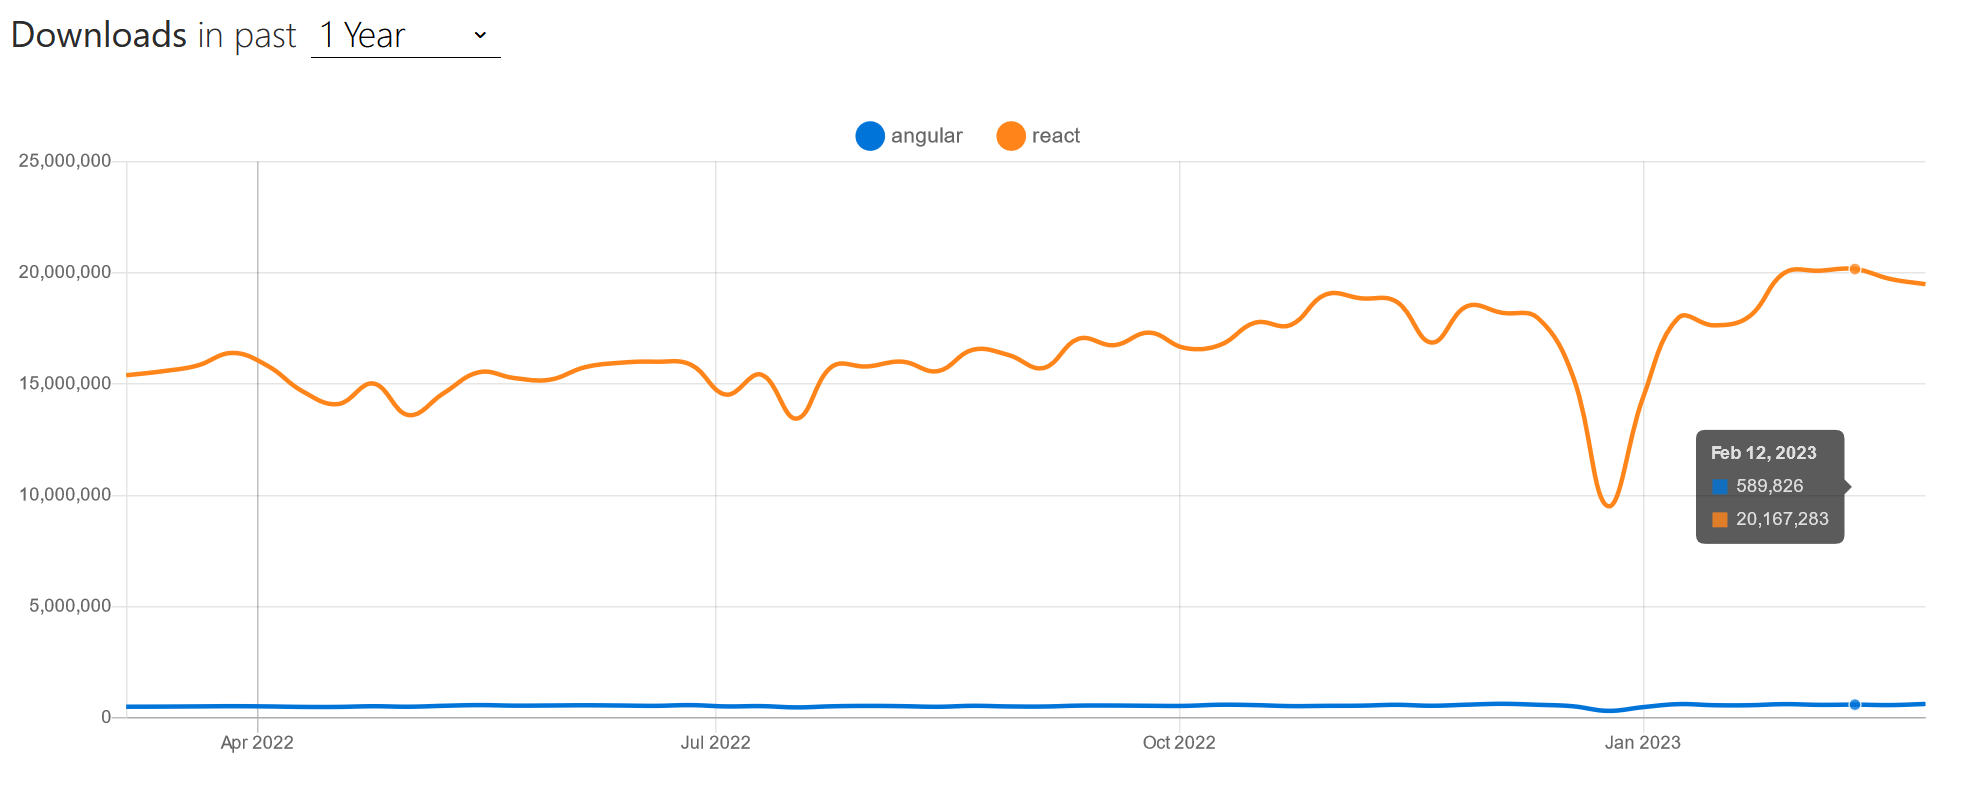
\includegraphics[width=1\textwidth]{pics/WebframeworkPopularity.png}
  \caption{Popularity of Web Frameworks}
  \label{fig:webpop}
\end{figure}
\\
Moreover, while we had some previous experience with JavaScript, we had never worked with TypeScript before, which made the attempt 
to understand Angular even more difficult than it needed to be. The comparatively better scalability of Angular was also not needed
for our project as it not likely to expand and therefore need for resources in the future.

\section{Next.js}
\setauthor{Christoph Lasinger}
Next.js is a React framework, meaning that, while React provides functions and features to build user interface elements
as a JavaScript library, Next.js handles the configuration and tooling that React needs. Additionally, Next.js provides
new features, structures, and optimizations. These additional features include data fetching, integrating, routing,
and so on \cite{NextjsDescription}.
\\
\subsection{Pages}
\setauthor{Christoph Lasinger}
One feature of Next.js that one will notice immediately is the representation of a webpage in JavaScript (or TypeScript) files as
so-called pages. In essence, they are React components that correlate to a route according to their file name (dynamic routing) and
have certain behaviours built into them from the moment of their creation.

For example, by default every page is pre-rendered, meaning that the HTML code of a webpage and as little JavaScript code as possible
that is required to perform its functions is generated in advance, instead of it having to be built from the JavaScript source code by
the client. This results in better performance and improves SEO, which means Search Engine Optimization and describes the process
of improving one's website in order to increase its visibility to search engines (e.g., Google).

In terms of implementing pre-rendering Next.js offers two general approaches: 
\begin{itemize}
  \item Static generation, which generates the HTML code for a webpage once when it is built and reuses it when responding to any request after that
  \item Server-side rendering, SSR for short and also referred to as dynamic rendering, which generates the HTML code anew each time a request is made
\end{itemize}

Next.js offers the option to use either one of these pre-rendering
techniques or both in combination, where most pages are statically generated, and others are rendered on the server. In its official
documentation Next.js recommends the usage of static generation over SSR because of its better overall performance. However, server-side
rendering might be necessary in some cases, for example when some data that is fetched from an API and displayed on the website needs
to be frequently updated \cite{NextjsPages}.
\\
\subsection{Data fetching}
\setauthor{Christoph Lasinger}
When developing a website, it is common to need to frequently fetch data from a remote source in order to update whatever is displayed
on the website. Because data fetching can play such an important role, Next.js offers several different ways to do it, that one can choose
from depending on the specific requirements and use cases of one's application. As server-side rendering and static-site generation have already
been thoroughly explained, the focus of this paragraph lies on the other two methods instead, though it should be noted that they are used by
exporting a function called \emph{getServerSideProps} or \emph{getStaticProps} respectively.

In contrast to server-side rendering, Next.js also offers the
option of client-side rendering or client-side data fetching, where data is generally fetched at runtime and at the component level. As a
result, the content of a page only changes whenever new data comes in. Though this can negatively affect performance and load time of one's
website, client-side rendering can be useful when SEO is not of importance, and pages need to be updated very frequently based on fetched data.
For implementing this strategy Next.js offers the React hook library SWR (stale-while-revalidate), a cache invalidation strategy
of HTTP. Next.js strongly encourages developers to use it in its documentation, as it handles focus tracking, caching, revalidation, etc. The
other method of data fetching is called ISR (Incremental Static Regeneration) and allows developers to statically generate pages on a
per-page basis, without the need of rebuilding the entire website. In order to use it, a revalidate prop is added to the \emph{getStaticProps} function \cite{NextjsDataFetching}.
\\
\subsection{Code splitting}
\setauthor{Christoph Lasinger}
Another feature of Next.js is called code splitting, which is the process of splitting the bundle of an application into multiple smaller parts
required by each entry point, an entry point usually being a page. This is done in order to be able to only load the code required to run the one
page that is being viewed at the time, reducing the initial load time of the website as a result. It is to note that any code shared between pages
is split into separate bundles in order to have everything available that is needed to load a page. Additionally, Next.js makes it possible to
pre-load the code of pages that users commonly navigate to next, further improving user experience \cite{NextjsCodeSplitting}.
\\
\subsection{Image optimization}
\setauthor{Christoph Lasinger}
When it comes to performance Next.js offers a special Image component that extends the default image HTML element and should be used instead of
it as it has several advantages. For one, because of its performance optimizations and improved Core Web Vitals, metrics provided by Google that
measure end-user page experience, using Image components improves SEO. These optimizations include automatically serving images in their correct
size, resizing them on-demand if it is needed, and in modern formats, providing visual stability i.e., preventing the layout from shifting unexpectedly
and potentially causing errors, only actually loading the image if it can be seen by the user, etc. The actual images can be either stored locally
or loaded remotely and if there is an image on page that is especially important, perhaps very big or noticeable if absent, it can be given priority
when being loaded \cite{NextjsImageOptimization}.
\\
\subsection{Conclusion}
\setauthor{Christoph Lasinger}
After starting out with Angular and then switching to React, we ultimately decided to use Next.js for a number of reasons. For example, the built-in
routing system, very easy setup through the create-next-app command, aforementioned features that increase performance, the simplicity of its
file structure, namely all pages being in one folder, and so forth. Especially the gentleness of its learning curve had a big influence on the decision.

\section{Sass}
\setauthor{Christoph Lasinger}
Sass stands for syntactically awesome style sheets and is a stylesheet language that compiles into CSS (Cascading Style Sheets). It extends CSS by a number
of features such as functions, variables, nested loops, mixins, etc. As a result, Sass enables stylesheets to be organized more easily and for design
to be shared within and across projects. There are two syntactic variants i.e., versions of Sass, the most commonly used one being the SCSS syntax, where the
filename ends in .scss. It is a superset of CSS, meaning that all CSS code is also valid SCSS code. The other version of Sass is called the Sass syntax
and is a bit more unusual i.e., sort of like the programming language Python it abandons the typical structure of curly braces and semicolons used in CSS
to separate and organize lines of code in favour of simple indents and newlines. However, apart from the different styling elements used, both syntaxes
are the same in all other aspects, including the features they provide. Since SCSS is a superset of CSS, one can simply write CSS code for the most part
and use any SCSS feature when it seems useful, which makes Sass very easy to learn and adopt \cite{SassFeatures}.
\\
\subsection{Variables}
\setauthor{Christoph Lasinger}
For example, instead of copying the hexadecimal value representing a colour for each and every element and possibly making mistakes, Sass makes it possible
to store the colour code in a variable and access it using its more human-readable name. This feature can be very useful when for example working with brand
colours or main themes, as in those cases it is important to consistently use the exact same colour each time \cite{SassFeatures}.
\\
\subsection{Inheritance}
\setauthor{Christoph Lasinger}
Another useful feature of Sass is inheritance, an example of which can be seen in the following code snippet \ref{lst:sass}.

\begin{lstlisting}[language=Python,caption=Textstyling in Sass,label=lst:sass]
  .default_text{
    text-align: center;
    color: white;
    font-family: Prototype;
  }

  .legal_notice_text{
    @extend .default_text;
    font-size: 0.5em;
  }
\end{lstlisting}

Through the \emph{extend} keyword CSS properties of one selector can be passed over to another selector which then automatically has the 
same properties set to the same values, thus inheriting them. In this example, legal-notice-text is merely a variant of the 
default-text and should therefore be of the same colour, font, and alignment. However, as legal-notice-text is of not much 
importance to the average user of the website, it should be rather small and take up little space. Because of the usage of 
inheritance, the code becomes more readable and easier to write and understand \cite{SassFeatures}.
\\
\subsection{Partials}
\setauthor{Christoph Lasinger}
When working on a very large project with a lot of different people file management and organization can certainly become difficult. In
these cases the partials feature of Sass can be of great use. It allows the separation of one big Sass file into multiple smaller ones,
thus modularizing it. These smaller files usually have names ending in \emph{(\_partials.scss}, where the underscore marks the file as one
that is not to be converted to a CSS file, and can be used in any other Sass files with the usage of the @use rule \cite{SassFeatures}.
\\
\subsection{Nesting}
\setauthor{Christoph Lasinger}
Other, smaller features of Sass include nesting, where multiple CSS selectors can be written under one, overarching selector creating a
clear visual hierarchy like in HTML, and the ability to use mathematical operators when for example calculating the width of a HTML
element, making the CSS more readable and the thought process behind certain values clearer, than simply using a specific number, like
575 pixels. There are also so-called mixins, basically reusable CSS selectors that can be customized in a specific instance by passing it
variables as parameters, that can be created using the @mixin rule and used with the @include rule \cite{SassFeatures}.
\\
\subsection{Conclusion}
\setauthor{Christoph Lasinger}
Overall, Sass has many useful features that in some cases can make a very big difference in terms of readability, level of organization and
convenience when writing CSS with no real downsides. Since Next.js has built-in support for Sass it is very simple to install and use right
away. For these reasons we decided to use Sass, specifically the SCSS syntax, for our project Animotion \cite{NextjsCSSSupport}.
\\
\section{Comparison of 3D rendering technologies}
\setauthor{Romeo Bhuiyan}
In order to display a virtual model on a canvas, a 3D rendering technology was required. Two libraries, 
GLTFLoader and WebGL, were evaluated using JavaScript to determine the best fit for the task at hand. 
The choice between the two ultimately depends on the specific needs and limitations of the project. 
Both GLTFLoader and WebGL are effective tools for rendering, but each have their own 
unique strengths and weaknesses.

\subsection{WebGL}
\setauthor{Romeo Bhuiyan}
\textbf{WebGL} is designed to work seamlessly with other web technologies such as HTML, CSS, and JavaScript, 
making it easy to integrate 3D graphics into web pages. It allows developers to create a wide range 
of interactive 3D applications and visualizations, including games, scientific 
simulations, data visualizations, and more.
One of the key features of WebGL is its ability to take full advantage of the GPU 
(graphics processing unit) on the user's device. This allows WebGL applications to 
run smoothly and efficiently, even on devices with limited resources. Additionally, WebGL provides 
a high level of compatibility across different browsers and devices, making it a widely accessible technology.
WebGL is supported by most modern web browsers, including Chrome, Firefox, Safari, and Edge. 
This means that developers can create WebGL applications that can be easily accessed by 
users on a wide range of devices and platforms. \cite{WebGL}

\subsection{GLTFLoader}
\setauthor{Romeo Bhuiyan}
\textbf{GLTFLoader} is a JavaScript library that allows developers to load and parse 3D models in the GLTF 
(GL Transmission Format) file format. GLTF is a widely adopted file format for 3D models and is 
supported by many 3D modeling software, including Blender and SketchUp.
GLTFLoader provides a simple and easy-to-use API for loading and parsing GLTF models, 
which can then be displayed using WebGL. The library takes care of all the complex tasks 
involved in loading and parsing the model data, such as handling binary buffers, parsing 
JSON data and creating the geometry and materials for the model.
GLTFLoader also provides support for advanced features such as animations, skinning and morph 
targets, which are typically found in more complex 3D models. This allows developers to create 
more advanced and interactive 3D applications and visualizations.
One of the key benefits of using GLTFLoader is that it greatly simplifies the process of loading and 
displaying 3D models on the web. By using a standardized file format and a dedicated library, 
developers can focus on creating the logic and functionality of their application, rather than 
spending time on complex parsing and loading tasks.
Additionally, GLTF is a highly efficient format, which means that it can be loaded faster, 
and also the files are smaller in size, making it a great choice for loading 3D models on the web. \cite{GLTFLoader}

\subsection{Conclusion}
In conclusion, GLTFLoader is a powerful tool for creating 3D graphics for the web that 
offers several advantages over WebGL. One of the main benefits of using GLTFLoader is 
its ability to handle the loading and parsing of GLTF (GL Transmission Format) files, 
which are a widely-used format for 3D models. This eliminates the need for developers 
to write their own code to handle file loading and parsing, saving time and effort. 
Additionally, GLTFLoader provides a more streamlined and convenient way to work with 
3D models, as it allows developers to easily import and use pre-existing models rather 
than having to create them from scratch. Furthermore, GLTFLoader also supports various 
features such as animations, cameras, lights and many more which can be easily integrated 
with web pages. Therefore, it is more efficient and convenient for the purpose of Animotion 
to work with 3D models on the web, GLTFLoader is the best choice as seen below in the figure. \ref{fig:gltfloader}
\\
\begin{figure}[htb]
    \centering
    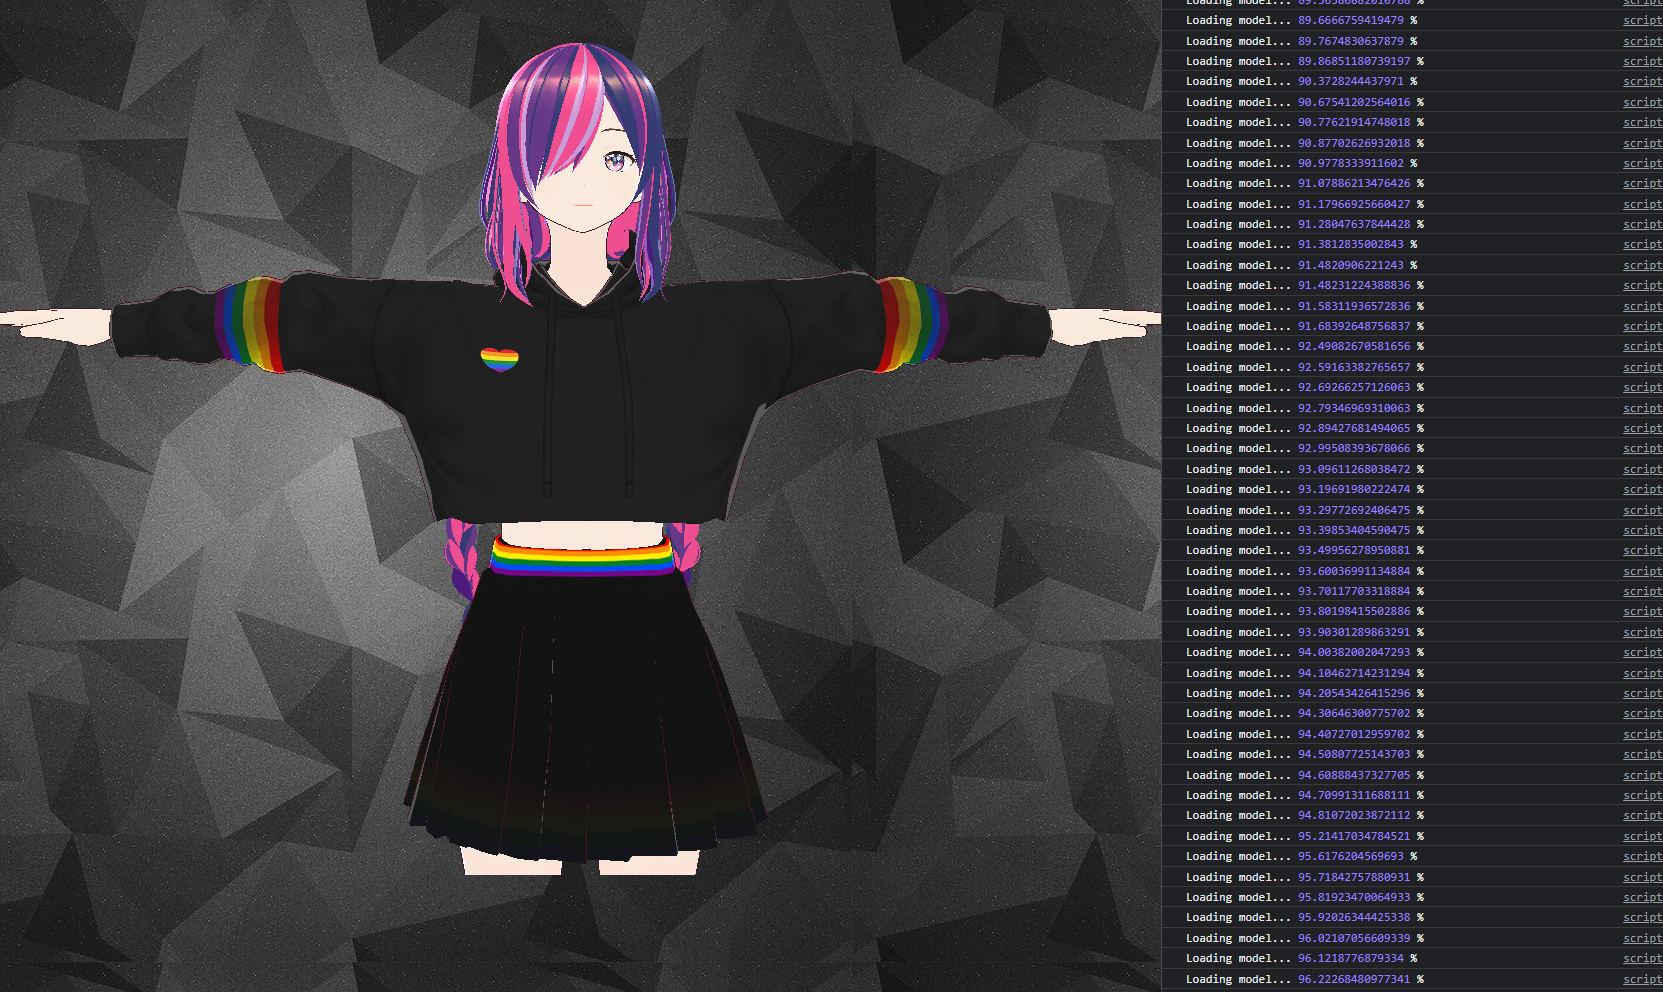
\includegraphics[width=0.9\textwidth]{pics/GLTFLoader.png}
    \caption{Loading the model with the help of GLTFLoader}
    \label{fig:gltfloader}
\end{figure}
\newpage
\section{Object interaction with OrbitControls}
\author{Romeo Bhuiyan}
\textbf{Orbit-Controls.js} is a JavaScript library used for controlling camera rotations 
and movements in 3D graphics applications. This library provides an easy-to-use 
interface for controlling the camera in a 3D environment, and is commonly used in 
interactive 3D web applications and other 3D visualizations.

The library works by allowing the user to control the camera through mouse 
and touch inputs, such as panning, zooming, and rotating the camera around a 
certain point in the 3D space. It uses the Three.js library, which is a popular 
library for creating 3D graphics in the browser, as a base.

Orbit-Controls.js makes it easy to interact with 3D scenes and view them from different 
perspectives. It provides a simple way to navigate and explore 3D environments, making it a 
useful tool for a wide range of applications, including scientific simulations, product visualization, architecture, and more.

The Orbit-Controls.js is a JavaScript library that enables user interactivity in 3D scenes built with Three.js. 
In order to use the library, it is necessary to include it in the HTML file and create an instance of the 
OrbitControls class. A Three.js camera object and a renderer also need to be passed as parameters. Once initialized, 
the library will handle user inputs from mouse and touch, allowing for smooth camera control in the 3D scene. 
This feature makes Orbit-Controls.js a valuable tool for creating interactive and engaging web applications with Three.js. \cite{orbitcontrols}

\subsection{Azimuth- and polar angle}
\setauthor{Romeo Bhuiyan}
The \textbf{Azimuth angle and the Polar angle} are two important concepts in 3D graphics and visualization. 
In the context of orbit-controls.js, they are used to control the camera's rotation and position in 3D space.

The Azimuth angle refers to the angle between a reference plane and the position of the camera in 
the x-z plane. This angle determines the camera's horizontal rotation and the direction it is facing. 
In orbit-controls.js, the Azimuth angle is controlled by moving the mouse horizontally.
The equation is given by: \ref{eqn:azimuth}
\begin{equation}
  \label{eqn:azimuth}
	azimuth = atan2(sin(\theta), cos(\theta)*sin(\phi) - tan(\phi)*cos(\theta))
\end{equation}
where theta represents the angle of inclination, measured from the horizontal, and phi represents the angle 
of rotation around the vertical axis, measured from the north.

The equation involves several trigonometric functions, including sin, cos, and tan, which describe the various 
components of the angle of inclination and rotation. The atan2 function is used to calculate the angle between 
the positive x-axis and the point (sin(theta), expression in parentheses) in the Cartesian plane.

The azimuth angle is an important parameter in many applications, including navigation, surveying, and satellite communications. 
It provides a convenient way to describe the direction of an object or location relative to true north, 
and can be used to determine the angle of elevation and other important parameters.

The Polar angle, on the other hand, refers to the angle between the position of the camera and the 
positive y-axis. It determines the camera's vertical rotation and the height of the camera relative 
to the scene. In orbit-controls.js, the Polar angle is controlled by moving the mouse vertically.
The polar angle, denoted by theta, is an angular coordinate system used in two-dimensional space to locate 
a point using a distance (r) and an angle (theta) measured from a fixed reference point.

It is the angle between the positive x-axis and the line segment 
joining the origin and the point (r, theta). The angle theta is measured in a counterclockwise direction 
from the positive x-axis, ranging from 0 to 2pi radians (or 0 to 360 degrees). The equation is: \ref{eqn:polar}
\begin{equation}
  \label{eqn:polar}
  \theta = arctan(y/x)
\end{equation}
where (x,y) are the Cartesian coordinates of a point in the plane. This equation finds the angle between the positive x-axis 
and the line segment connecting the origin and the point (x, y).
It is important to note that this formula works only when x is positive. If x is negative, 
then we must add or subtract pi radians (180 degrees) to the result, depending on the sign of y, to find the correct angle.

By controlling both the Azimuth and Polar angles, the orbit-controls.js library allows the user to 
change the position and orientation of the camera in 3D space. This is especially useful for interactive 
3D visualizations, where the user needs to be able to explore the scene from different perspectives, as shown below in the figure. \ref{fig:orbitcontrols}

Orbit-controls.js is often used in conjunction with WebGL and Three.js, which are libraries for creating 
3D graphics and animations in the browser. The combination of these technologies makes it possible to create 
interactive 3D visualizations that can run in a web browser, without the need for additional software or plugins.
\\
\begin{figure}[htb]
  \centering
  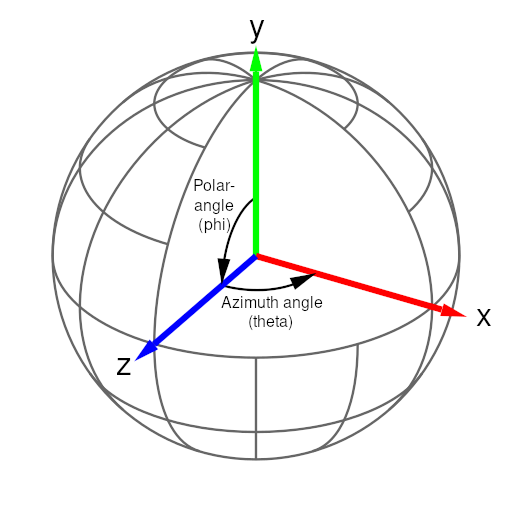
\includegraphics[width=0.5\textwidth]{pics/orbitcontrols.png}
  \caption{Azimuth and Polar angle}
  \cite{angles}
  \label{fig:orbitcontrols}
\end{figure}

\section{Camera utilization using camera utils}
\setauthor{Romeo Bhuiyan}
The \textbf{camera utils.js} library is a JavaScript-based tool for controlling camera behavior in web-based applications. 
This library provides a set of functions and utilities that simplify the process of integrating camera functionality 
into a web application. By leveraging the camera utils.js library, developers can add camera-based features to 
their web applications with ease and efficiency.

The camera utils.js library provides a simple and intuitive interface for controlling camera movements and behaviors 
in web-based applications. With this library, developers can specify camera movement and behavior through a simple 
set of functions and parameters, rather than having to manually manipulate camera coordinates and behaviors. 
This makes it easier for developers to create rich and immersive camera experiences in their web applications.

One of the key benefits of using the camera utils.js library is that it enables developers to take advantage of 
modern web-based technologies, such as WebRTC and WebGL, to create camera-based experiences. These technologies 
allow developers to access the user's camera in real-time, making it possible to create live-streaming and 
real-time interactive experiences. By using the camera utils.js library, developers can take advantage of these 
technologies to create engaging and interactive camera-based experiences that work seamlessly across a wide range of devices and browsers.
In addition to providing a simple and intuitive interface for controlling camera behavior, the camera utils.js 
library also offers a number of performance and optimization optimizations that help to ensure smooth and fast 
camera performance. For example, the library implements a number of techniques to reduce latency and ensure 
smooth camera movement, even when processing large amounts of data in real-time.

\section{Drawing utils}
\setauthor{Romeo Bhuiyan}
\textbf{drawing utils.js} is a JavaScript library designed to simplify and streamline the process of 
creating and rendering graphics within a web-based environment. The library provides a set of utility 
functions that enable developers to quickly and easily implement common graphical tasks such as 
creating 2D shapes, generating text, and creating animations.

One of the key benefits of using drawing utils.js is that it abstracts away much of the 
low-level graphics programming that would otherwise be required to achieve these same results. 
This means that developers can focus on the high-level aspects of their project and get the 
desired results more quickly and efficiently. Additionally, the library provides a set of 
well-documented and easy-to-use APIs that enable developers to implement and customize 
their graphics with minimal effort.

In terms of its usage, drawing utils.js can be utilized in a variety of web-based projects, 
including virtual reality (VR) and augmented reality (AR) applications, gaming engines, 
and data visualization tools. It is particularly useful for those looking to build complex 
and sophisticated graphics-intensive applications, as it provides a comprehensive set of 
tools and functions that can help to simplify and optimize the development process.

In the context of our VRM model program, drawing utils.js is a valuable tool for 
creating, manipulating, and visualizing the graphical elements of the VRM model. 
It enables developers to quickly and easily create and render graphics, such as 
animations and 3D shapes, that are critical to the functioning and visual appeal 
of the VRM model. The library also provides a range of performance optimization 
features, such as caching and the ability to work with multiple GPUs, 
that can help to ensure that the VRM model runs smoothly and efficiently, even in demanding environments.

\section{Screen capture technology}
\setauthor{Romeo Bhuiyan}
Screen recording is an important aspect in the world of VRM programs. 
Screen recording allows for the capture of all the visual and audio elements that are displayed 
on a computer screen. The recorded content can then be shared, edited, and distributed for various 
purposes. In the context of Animotion, screen recording can serve several important functions.

First and foremost, screen recording can be used to document and showcase the functionality and 
capabilities of the VRM Model program. This can include recording the different animations, movements, 
and interactions that are possible within the program. This type of recording can be used to demonstrate 
the program's features to potential users, stakeholders, or clients, and can help to generate interest 
and engagement with the VRM Model program.

Screen recording can also be used to provide support and training to users of this kind of program. 
By recording step-by-step instructions or tutorials, users can learn how to use the program effectively, 
even if they have no prior experience or knowledge. Additionally, if users encounter any issues or 
difficulties while using the VRM Model program, a screen recording can be created to assist in resolving 
the problem and provide a visual representation of the issue at hand.

Screen recording can also be used to document bugs or other technical issues that arise during the use 
of the VRM Model program. By capturing the screen and audio output, developers and technical support 
teams can more easily diagnose and resolve any problems that may occur.
Lastly, screen recording can be used for creative purposes, such as creating animations or special 
effects using the VRM Model program. By capturing and manipulating the recordings, users can explore 
new ways to use and interact with the VRM Model program, and create new and unique content that 
can be shared and enjoyed by others.

\subsection{RecordRTC}
\setauthor{Romeo Bhuiyan}
\textbf{RTCRecord.js} is a JavaScript library that allows users to perform real-time communication (RTC) 
recording in the web browser. It uses the WebRTC API, which is a standardized way of enabling 
real-time communication capabilities in web browsers, to capture audio and video data from a 
user's microphone and webcam. The captured data can then be saved as a video file for future use.

One of the main use cases for RTCRecord.js is for screen recording in web-based applications, 
such as video conferencing and online collaboration tools. This allows users to record their 
screen activity, audio, and webcam footage in real-time, without the need for any additional 
software. The recorded videos can then be used for training purposes, for documentation, 
or for sharing information with others.

Another use case for RTCRecord.js is for creating educational content, such as tutorials 
and screencasts. With RTCRecord.js, users can easily record their screen and webcam footage, 
and share their knowledge with others in a visually engaging way. \cite{rtcrecord}

\subsection{FFmpeg}
\setauthor{Romeo Bhuiyan}
\textbf{FFmpeg} is an open-source software library for audio, video and image processing. 
The library can be used to encode, decode, transcode, mux, demux, stream, filter and play various 
multimedia files. It is written in the C programming language and is commonly used on a variety of 
operating systems including Windows, macOS, and Linux.

\texttt{FFmpeg.min.js} is a JavaScript implementation of FFmpeg, which can be used for client-side video 
processing in web applications. It provides a way for web developers to perform various multimedia 
operations in real-time within a web browser. With ffmpeg.min.js, developers can leverage the 
functionality of FFmpeg in their web applications, including video compression, resizing, cropping, and transcoding.

The library can be used for a range of purposes, including creating video editing tools, video 
compression utilities, and real-time video processing applications. With the rise of cloud computing, 
ffmpeg.min.js can be used to perform video processing operations in real-time on a server, without requiring 
the user to have FFmpeg installed on their local machine. This can save both time and resources, and provide 
a convenient solution for web developers looking to incorporate video processing capabilities into their applications. \cite{ffmpeg}

\subsection{WebM video format for web-based applications}
\setauthor{Romeo Bhuiyan}
The \textbf{WebM video format} is an open, royalty-free, and high-quality video compression format 
that has been specifically designed for the web. This format was developed by Google and 
the WebM Project, a community of developers and industry partners, with the goal of 
providing an alternative to proprietary video formats, such as \gls{h264} and \gls{mpeg}. 
The WebM format is based on the VP8 video codec and the Vorbis audio codec, 
which are both open-source and can be freely used without licensing fees.

One of the key benefits of the WebM format is its high-quality video compression, 
which provides visually lossless video playback without sacrificing file size. 
This makes WebM an ideal choice for multimedia applications that require 
high-quality video playback, such as video conferencing, video on demand, and live streaming. The format 
is also highly scalable and can be used on a wide range of devices, from desktop computers to mobile 
devices, ensuring compatibility across platforms.

Another important advantage of the WebM format is its compatibility with HTML5. The format is 
natively supported by most modern browsers, including Google Chrome, Mozilla Firefox, and Opera, 
and can be easily embedded into web pages without the need for additional plugins or software. 
This makes it an ideal choice for web-based video applications, as it eliminates the need for 
users to download and install additional software or plugins.

In addition to its compatibility and high-quality video compression, the WebM format also has 
a small file size, making it an ideal choice for applications that require fast loading times, 
such as online video platforms and websites. The format is also highly customizable, and developers 
can use the WebM SDK to modify and extend the format to meet their specific needs.
Another key benefit of the WebM format is its ability to support a wide range of video and audio 
codecs, including VP9, Opus, and VP10, making it a flexible choice for applications that require 
support for multiple codecs. The format also supports high dynamic range (HDR) video, providing 
users with a superior viewing experience with enhanced color and brightness. \cite{webm}

\section{Calculation of the virtual reality model} 
\setauthor{Romeo Bhuiyan}
Controlling a VRM on a website involves a complex process that involves 
capturing the user's inputs, updating the VRMs position and orientation in real-time, 
and rendering the updated model for display on the user's device.
The first step in this process is for the user to interact with the VR model 
using a device such as a VR headset or a mouse and keyboard. The inputs from the 
user are then captured by the website and sent to the server. The server then 
uses these inputs to update the VR model's position and orientation in real-time. 

Once the VR model has been updated, it is then rendered, and the new frame is 
sent back to the user's device for display. This process repeats as the user 
continues to interact with the VR model. 
To achieve this, various technologies are needed such as GLTFLoader from the three
libraries for rendering the VR model in the browser, WebSockets for real-time 
communication between the client and server, and a physics engine to simulate 
the movement and interactions of the VR model. 

\subsection{Blendshape}
\setauthor{Romeo Bhuiyan}
\textbf{Blendshape} is a technique used in 3D animation and computer graphics to create a smooth transition between different shapes or expressions of a 3D model. 
It works by creating a set of \emph{target} shapes for a 3D model, each representing a different expression or shape, 
and then using a set of weights or \emph{blend} values to interpolate between these target shapes, creating a 
smooth transition between them. This allows animators to create a wide range of expressive characters with a 
limited number of 3D models. Blendshapes are commonly used in animation, film and game industry.

\subsection{Lerp}
\label{sec:lerp}
\setauthor{Romeo Bhuiyan}
The \textbf{Lerp} function, short for Linear Interpolation, is a mathematical function that is 
used to smoothly blend between two values. The function takes three arguments: a start value, 
an end value, and a weight. The weight is a value between 0 and 1 that represents the proportion 
of the blend between the start and end values.
For example, if the weight is set to 0, the function will return the start 
value, and if the weight is set to 1, the function will return the end value. 
If the weight is set to 0.5, the function will return the midpoint between the 
start and end values. By adjusting the weight, the Lerp function can be used to 
smoothly transition between any two values over time.
In the context of computer graphics, Lerp function is widely used for 
interpolating values such as position, rotation, and color, to make the 
animation smooth. It's also used in physics simulations, game development, 
and other fields where the smooth transition of values is needed.

Mathematically explained the linear interpolation, or simply interpolation, 
is a technique used to estimate values between two known data points. In other words, given two data points, 
interpolation allows us to estimate the value of a function at any point between those two data points.
The formula for linear interpolation is given by: \ref{eqn:lerp}
\begin{equation}
  \label{eqn:lerp}
	y = y1 + (x - x1) * (y2 - y1) / (x2 - x1)
\end{equation}
This formula is used to estimate a value between two known values on a straight line. It requires the following variables: y, 
which represents the estimated value; y1, the value of the dependent variable (y-axis) at the first known point (x1, y1); y2, 
the value of the dependent variable at the second known point (x2, y2); x, the value of the independent variable (x-axis) 
at which to estimate the value of y; x1, the value of the independent variable at the first known point; and x2, the value 
of the independent variable at the second known point.

The linear interpolation formula calculates the value of y by first determining the slope of the line connecting the two 
known points (y1, x1) and (y2, x2), and then extrapolating from that slope to estimate the value of y at the point x. 
This method is commonly used in scientific research when estimating the value of a variable at a point where it has not 
been directly measured, but falls within a range of values for which measurements have been made.

\begin{figure}[htb]
  \centering
  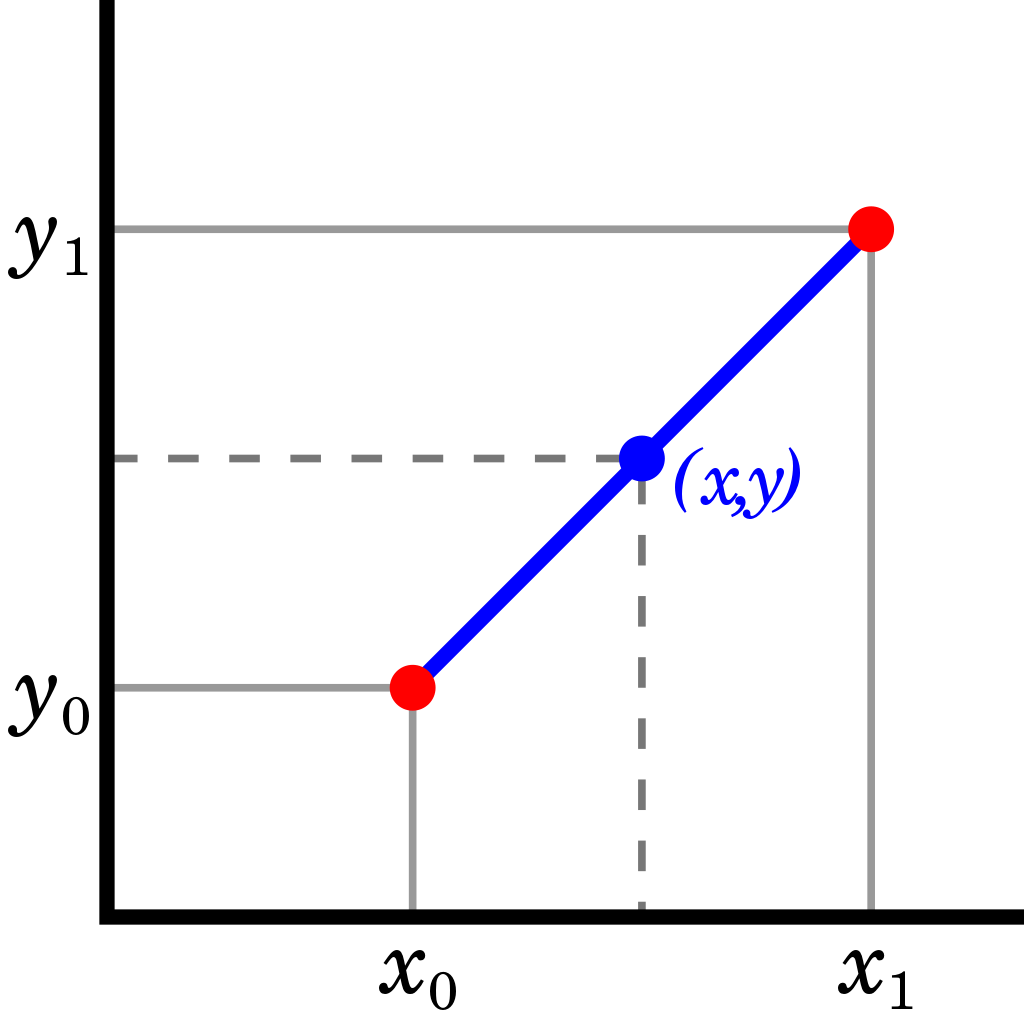
\includegraphics[width=0.4\textwidth]{pics/lerp.png}
  \caption{The blue line connecting the two red points is referred to as the linear interpolant, and it is used to estimate the value of y at a given x using linear interpolation.}
  \cite{angles}
  \label{fig:lerp}
\end{figure}

\subsection{Determining mouth expressions}
\setauthor{Romeo Bhuiyan}

\begin{lstlisting}[language=Python,caption=Shape of mouth,label=lst:shapeOfMouth]
    for each shape in ["I", "A", "E", "O", "U"]
        Blendshape.setValue(PresetName[shape], 
        lerp(riggedFace.mouth.shape[shape], 
        Blendshape.getValue(PresetName[shape]), 0.5))

\end{lstlisting}
As shown in the listing \ref{lst:shapeOfMouth}, this pseudocode is a loop that iterates over an array containing the shapes \texttt{A, E, I, O, U}. 
The purpose of the loop is to blend the shape of a rigged face's mouth with a preset value of a 
Blendshape object for each of these shapes. The loop starts by setting the value of the Blendshape 
object to a blended value between the shape of the rigged face's mouth \texttt{(riggedFace.mouth.shape[shape])}
and the current value of the Blendshape object \texttt{(Blendshape.getValue(PresetName[shape]))}. 
The blend is done using the lerp function, mentioned in above \ref{sec:lerp}. 
Quickly summarized, this function takes three arguments: the start value, the end value, and the weight of blending. 
In this case, the weight is set to 0.5, resulting in an even blend between the two values.
Once the blended value is calculated, it is set to the Blendshape object using the PresetName 
as the key. This process is repeated for each shape in the array, allowing the developer to 
easily blend the shape of the rigged face's mouth with preset values for multiple shapes.

\subsection{Blinking eyes}
\setauthor{Romeo Bhuiyan}
\begin{lstlisting}[language=Python,caption=Blinking of the eyes,label=lst:blinking]
    riggedFace.eye.l = lerp(clamp(1 - riggedFace.eye.l, 0, 1), Blendshape.getValue(PresetName.Blink), 0.5)
    riggedFace.eye.r = lerp(clamp(1 - riggedFace.eye.r, 0, 1), Blendshape.getValue(PresetName.Blink), 0.5)
    riggedFace.eye = Kalidokit.Face.stabilizeBlink(riggedFace.eye, riggedFace.head.y)
    Blendshape.setValue(PresetName.Blink, riggedFace.eye.l)

\end{lstlisting}
The pseudocode \ref{lst:blinking} shown above is a code block that performs blinking animation on a VRM model. 
The code uses the Lerp function, the clamp function, and the stabilizeBlink function 
to animate the eyes of the rigged face.

The first two lines of the code use the Lerp function to blend the current value of the left and right eye shapes 
\texttt{(riggedFace.eye.l and riggedFace.eye.r)} with a preset Blink value from the Blendshape object. The Lerp 
function takes the clamp of the inversed eye shape values \texttt{(1 - riggedFace.eye.l and 1 - riggedFace.eye.r)}, 
which clamps the values to between 0 and 1, and the preset Blink value, which is obtained using \texttt{Blendshape.getValue(PresetName.Blink)}. 
The weight of the blend is set to 0.5, resulting in an even blend between the two values.

The third line of the code stabilizes the blinking animation of the eyes by calling 
the stabilizeBlink function from the \texttt{Kalidokit.Face} module. This function takes the 
current eye shape \texttt{(riggedFace.eye)} and the head's y position \texttt{(riggedFace.head.y)}  as arguments 
and returns a stabilized eye shape.

Finally, the fourth line of the code sets the Blink value of the Blendshape object to the 
stabilized left eye shape \texttt{(riggedFace.eye.l)}. This will result in a smooth and stable blinking  
of the eyes on the VRM model.

In summary, this listing is a code block that animates the eyes of a VRM model by 
blending the current eye shape with a preset Blink value, stabilizing the blinking animation, 
and updating the Blink value of the Blendshape object. The code uses the Lerp function, the clamp 
function, and the stabilizeBlink function to create a smooth and stable blinking animation on the VRM model.

\subsection{Positioning the model}
\setauthor{Romeo Bhuiyan}

\begin{lstlisting}[language=Python,caption=Position of the model,label=lst:position]
    function rigPosition(name, position={x:0, y:0, z:0}, dampener=1, lerpAmount=0.3) {
        if (currentVrm is not defined) {
          return;
        }
        Part = currentVrm.humanoid.getBoneNode(name from THREE.VRMSchema.HumanoidBoneName);
        if (Part is not defined) {
          return;
        }
        vector = new THREE.Vector3(position.x * dampener, position.y * dampener, position.z * dampener);
        Part.position.lerp(vector, lerpAmount);
    }
      
      oldLookTarget = new THREE.Euler();
      function rigFace(riggedFace) {
        if (currentVrm is not defined) {
          return;
        }
        rigRotation("Neck", riggedFace.head, 0.7);
      
        Blendshape = currentVrm.blendShapeProxy;
        PresetName = THREE.VRMSchema.BlendShapePresetName;
    }
      

\end{lstlisting}
The pseudocode \ref{lst:position} about positioning is a code block that positions a VRM model according to a set of defined parameters. 
The code block consists of two functions: rigPosition and rigFace.

The \textbf{rigPosition function} takes three arguments: name, position, dampener, and lerpAmount. The name argument is the name 
of the part of the VRM model that needs to be positioned, the position argument is an object with x, y, and z properties 
that represent the desired position of the part, the dampener argument scales the position values, and the lerpAmount 
argument is the weight of the blend between the current position and the desired position.
The function starts by checking if the currentVrm is defined, and if it's not, the function returns without executing further code. 
If currentVrm is defined, the code uses the \texttt{humanoid.getBoneNode} method to retrieve the part specified by the name argument. 
If the part is not defined, the function returns without executing further code.
If the part is defined, the code creates a new \texttt{THREE.Vector3} object with the desired position 
values (scaled by the dampener argument), and the Part.position property is blended towards the 
desired position using the lerp method. The weight of the blend is set by the lerpAmount argument.

The \textbf{rigFace function} takes one argument: riggedFace, which represents the face of the VRM model. The function starts 
by checking if the \emph{currentVrm} is defined and if it's not, the function returns without executing further code.
If \emph{currentVrm} is defined, the function calls the rigRotation method and passes two arguments: \emph{Neck} and \emph{riggedFace.head}, 
with a third optional argument of 0.7. This rotates the neck of the VRM model according to the head position.
The function also defines the Blendshape variable and assigns it to the \texttt{blendShapeProxy} property of the \emph{currentVrm} object. 
The \texttt{PresetName} variable is set to the \texttt{BlendShapePresetName} property from the \texttt{THREE.VRMSchema} object.

\subsection{Animating the body}
\setauthor{Romeo Bhuiyan}
\begin{lstlisting}[language=Python,caption=Animating the rest of the body,label=lst:restbody]
    if (pose2DLandmarks && pose3DLandmarks) {
    riggedPose = solvePose(pose3DLandmarks, pose2DLandmarks, "mediapipe", videoElement);
    rotate("Hips", riggedPose.Hips.rotation, 0.7);
    position("Hips", -riggedPose.Hips.position.x, riggedPose.Hips.position.y + 1, -riggedPose.Hips.position.z, 1, 0.07);

    rotate("Chest", riggedPose.Spine, 0.25, 0.3);
    rotate("Spine", riggedPose.Spine, 0.45, 0.3);

    rotate("RightUpperArm", riggedPose.RightUpperArm, 1, 0.3);
    rotate("RightLowerArm", riggedPose.RightLowerArm, 1, 0.3);
    rotate("LeftUpperArm", riggedPose.LeftUpperArm, 1, 0.3);
    rotate("LeftLowerArm", riggedPose.LeftLowerArm, 1, 0.3);

    rotate("LeftUpperLeg", riggedPose.LeftUpperLeg, 1, 0.3);
    rotate("LeftLowerLeg", riggedPose.LeftLowerLeg, 1, 0.3);
    rotate("RightUpperLeg", riggedPose.RightUpperLeg, 1, 0.3);
    rotate("RightLowerLeg", riggedPose.RightLowerLeg, 1, 0.3);
}

\end{lstlisting}
The listing \ref{lst:restbody} shown above, describes an animation process for a VRM body. 
The code checks if the \emph{pose2DLandmarks} and \emph{pose3DLandmarks} are available. If they are both available, 
the code calculates the rigged pose using the function \texttt{solvePose} with the \texttt{pose3DLandmarks}, \texttt{pose2DLandmarks}, 
\texttt{mediapipe}, and \texttt{videoElement} as input parameters. The function \texttt{solvePose} returns the rigged pose, which 
is then stored in the variable \texttt{riggedPose}.
The code then rotates and positions various body parts of the VRM model based on the values obtained from the 
rigged pose. For example, the hips are rotated based on the value of \texttt{riggedPose.Hips.rotation} with a weight 
of 0.7, and their position is changed to \texttt{x: -riggedPose.Hips.position.x, y: riggedPose.Hips.position.y + 1, z: 
-riggedPose.Hips.position.z} with a weight of 1 and a smoothing factor of 0.07. Similar operations are performed 
for the chest, spine, arms, and legs.
The rotation and position of each body part is performed using two separate functions: \texttt{rotate} and 
\texttt{position}. The first parameter of each function specifies the name of the body part to be animated, 
while the remaining parameters specify the values used for rotation or position, weight, and smoothing factor.
In this way, the VRM model's body is animated according to the solved pose information.

\subsection{Animation of both hands}
\setauthor{Romeo Bhuiyan}
\begin{lstlisting}[language=Python,caption=Animating the left hand,label=lst:hands]
    if (leftHandLandmarks) {
        # Obtain the rotation information of the left hand
        riggedLeftHand = Hand.solve(leftHandLandmarks, "Left");
      
        # Apply the rotation to the left hand rig
        rigRotation("LeftHand", {
          z: riggedLeftHand.LeftWrist.z,
          y: riggedLeftHand.LeftWrist.y,
          x: riggedLeftHand.LeftWrist.x,
        });
      
        # Apply the rotation to each of the finger bones
        rigRotation("LeftRingProximal", riggedLeftHand.LeftRingProximal);
        rigRotation("LeftRingIntermediate", riggedLeftHand.LeftRingIntermediate);
        rigRotation("LeftRingDistal", riggedLeftHand.LeftRingDistal);
        rigRotation("LeftIndexProximal", riggedLeftHand.LeftIndexProximal);
        rigRotation("LeftIndexIntermediate", riggedLeftHand.LeftIndexIntermediate);
        rigRotation("LeftIndexDistal", riggedLeftHand.LeftIndexDistal);
      }
\end{lstlisting}
The provided pseudocode \ref{lst:hands} animates the left (same for the right) hand of a VRM character. 
It starts by checking if the left hand landmarks have been detected. 
If they have, the code then calculates the rotations of the left hand by 
using the \texttt{Hand.solve} function, which takes in the left hand landmarks and the string \texttt{Left}.
The resulting rotations are then applied to the left hand rig and each of the finger 
bones using the \texttt{rigRotation} function. For the left hand rig, the function is called with 
the string \texttt{LeftHand} and the rotation values for the x, y, and z axes, obtained from the 
\texttt{riggedLeftHand} object.
Similarly, the rotations of each finger bone are applied by calling the \texttt{rigRotation} function 
with the names of the bones, such as \texttt{LeftRingProximal},\texttt{LeftRingIntermediate}, and \texttt{LeftRingDistal}, 
and the corresponding rotation values obtained from the \texttt{riggedLeftHand} object. The same process is 
repeated for each of the other finger bones.